\documentclass[12pt]{article} 
\usepackage{graphicx}
\usepackage[utf8]{inputenc} 
\usepackage{listings}
\usepackage{hyperref}

\title{\textbf{Labwork 4: Image Grayscale Conversion using CUDA}}
\author{Truong Quang Nam\\Student ID: 2540080}
\date{\today}

\begin{document}
\maketitle

\section{System Specifications}
\begin{itemize}
    \item \textbf{GPU:} NVIDIA GeForce GTX 1650
    \item \textbf{CPU:} AMD Ryzen 7 4800H
\end{itemize}

The original color image used for testing and processing is shown in Figure~\ref{fig:mo_ta_anh}.
\begin{figure}[htbp]
    \centering
    \includegraphics[width=0.7\textwidth]{Image.jpg}
    \caption{Original input color image}
    \label{fig:mo_ta_anh}
\end{figure}

\section{GPU Compute 2D}
This section details the implementation of converting the color image "Image.jpg" into a grayscale image using the GPU via Numba CUDA.

\subsection{Kernel Implementation}
The execution step uses a 2D grid structure where each thread calculates the grayscale value for a single pixel:
\begin{verbatim}
@cuda.jit
def gray_image(image_flat, gray_flat, height, width):
    x, y = cuda.grid(2)

    if x < width and y < height:
        r = image_flat[y, x, 0]
        g = image_flat[y, x, 1]
        b = image_flat[y, x, 2]

        gray_flat[y, x] = (r + g + b) / 3.0
\end{verbatim}

\subsection{Memory Allocation and Kernel Launch}
First, the input image data is transferred from the host (CPU) memory to the device (GPU) memory, and an empty device array is allocated for the output:
\begin{verbatim}
d_img_flattened = cuda.to_device(img_float)
d_gray_flattened = cuda.device_array((height, width), dtype=np.float32)
\end{verbatim}

Next, the thread blocks and grid layout dimensions are defined to invoke the execution configuration. We synchronize the stream to ensure accuracy before fetching results back to the host:
\begin{verbatim}
block_size = (32, 32)
grid_size = (8, 8)

gray_image[grid_size, block_size](
    d_img_flattened,
    d_gray_flattened,
    height,
    width
)
cuda.synchronize()
gray_flattened_cpu = d_gray_flattened.copy_to_host()
\end{verbatim}
The image rendering and saving components follow standard CPU procedures.

\section{Result}
The initial total computation block time recorded was around 463ms (including initial host-to-device memory allocation overhead). The resulting grayscale image is illustrated in Figure~\ref{fig:gpu}.

\begin{figure}[htbp]
    \centering
    \includegraphics[width=0.7\textwidth]{gray_image_gpu.png}
    \caption{Processed grayscale image output from GPU}
    \label{fig:gpu}
\end{figure}

\newpage
\section{Performance Analysis with Different Parameters}

To understand the scheduling impact, the kernel execution time was benchmarked over 1,000 iterations across various block dimensions.

\begin{figure}[htbp]
    \centering
    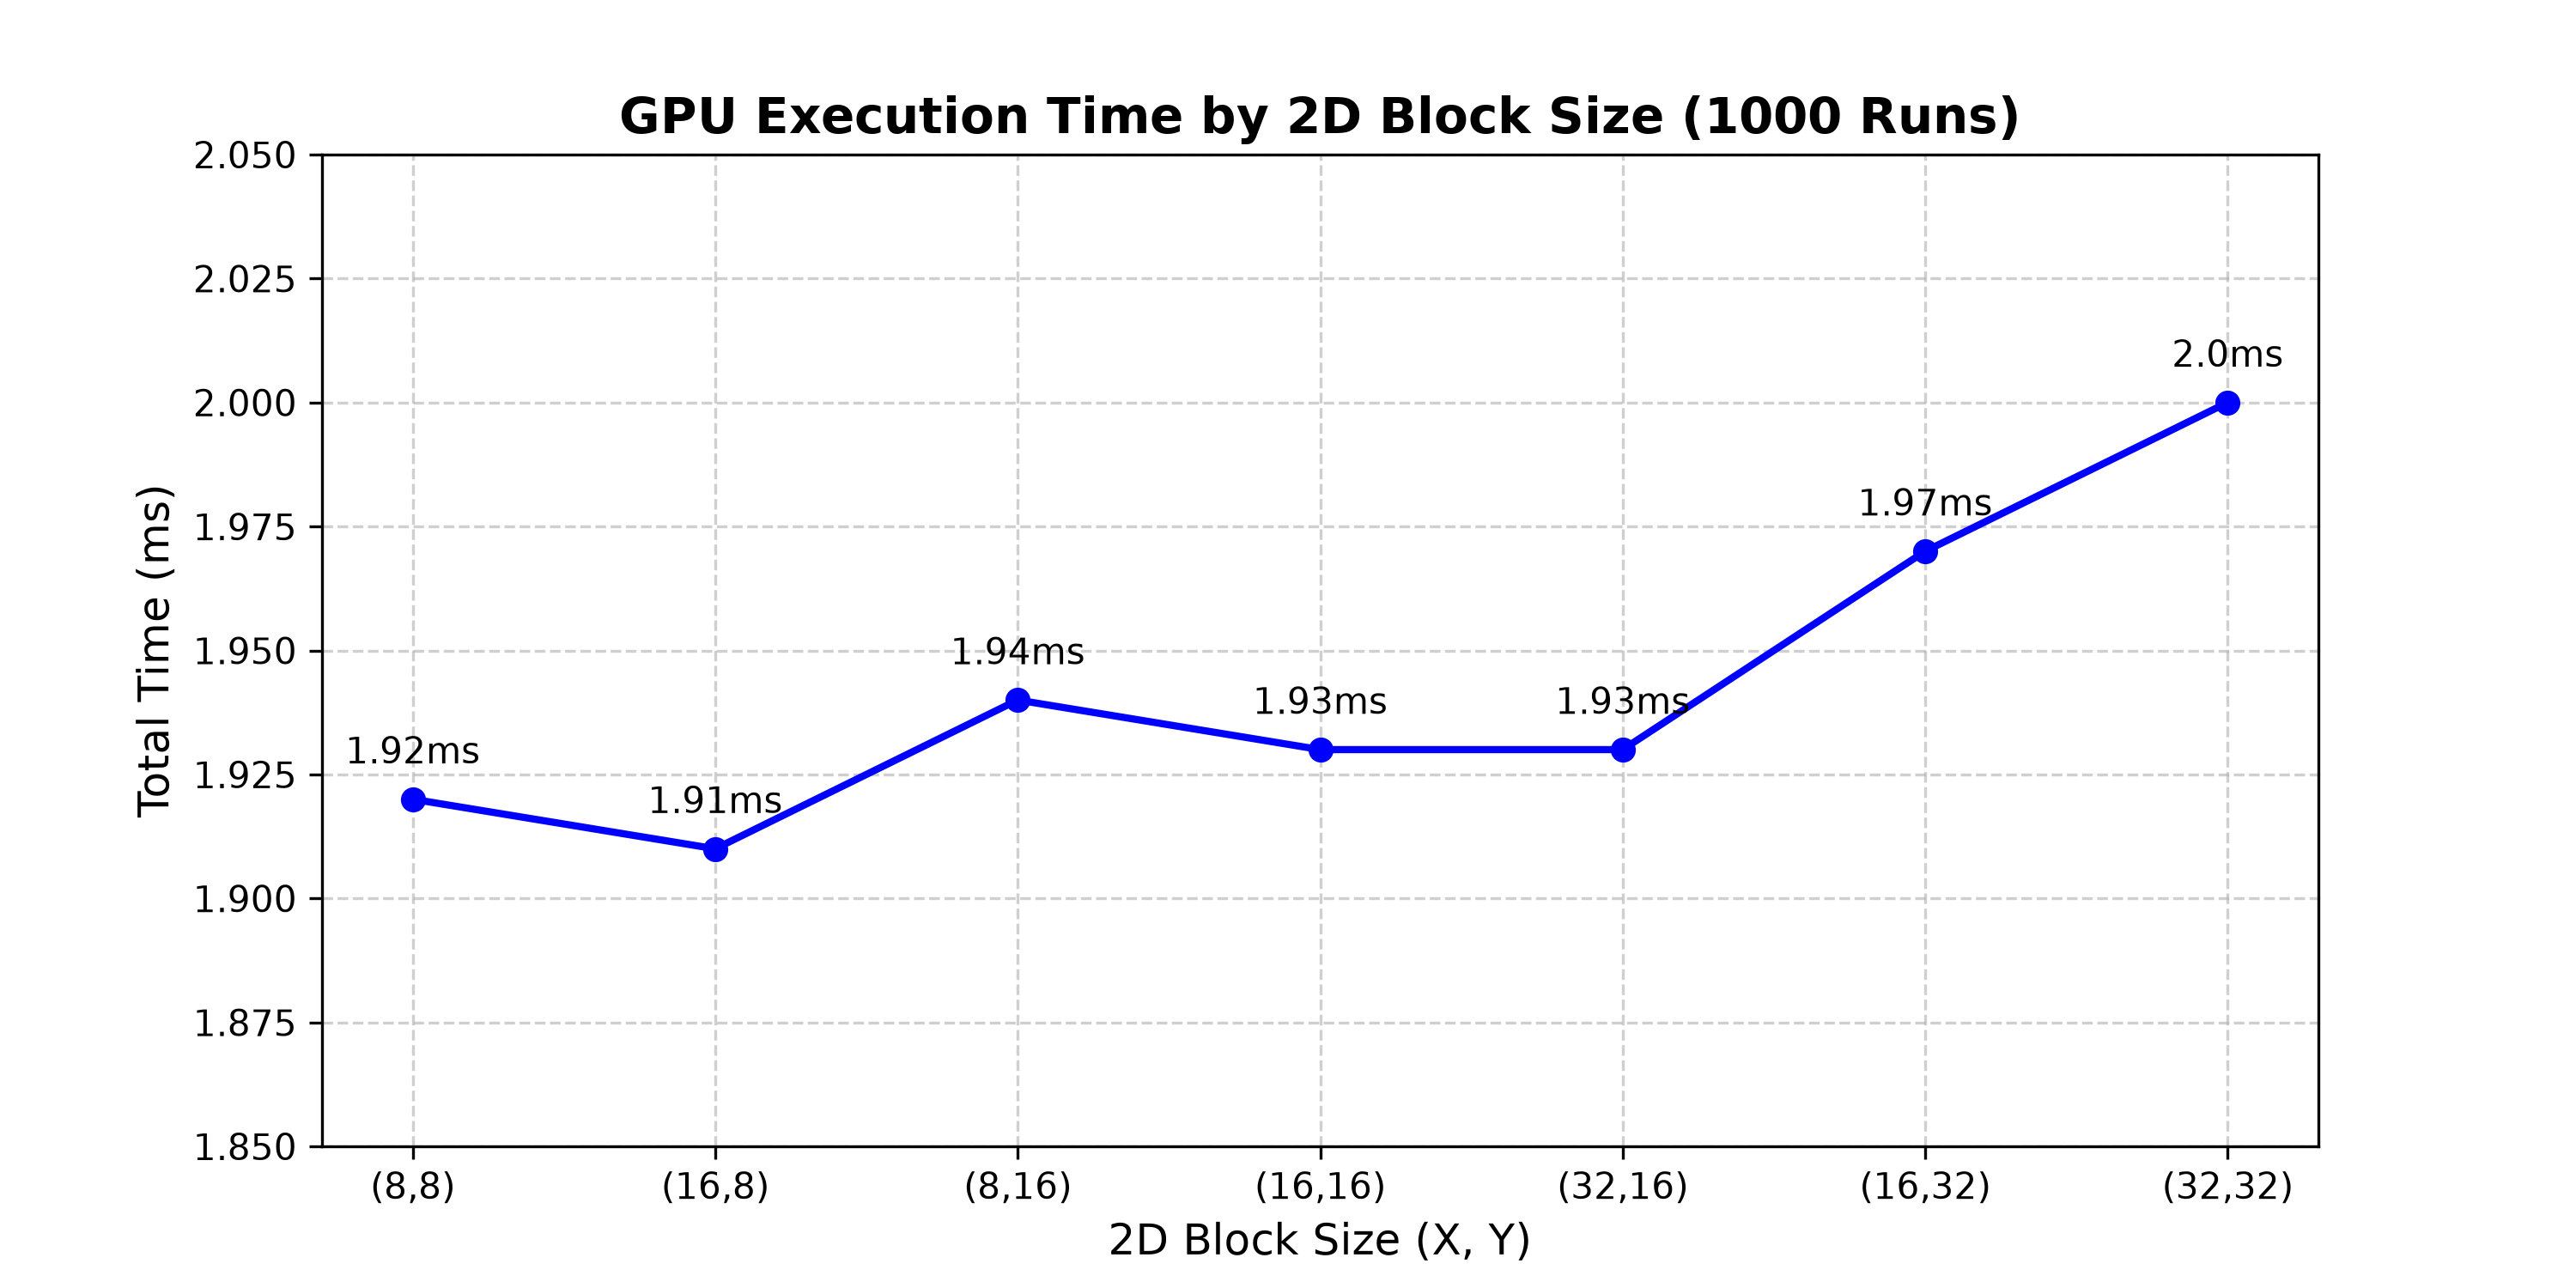
\includegraphics[width=0.75\textwidth]{gpu_performance_chart.png}
    \caption{GPU execution time across various 2D block size configurations}
    \label{fig:diff}
\end{figure}

As shown in Figure~\ref{fig:diff}, the most efficient block size configuration is \textbf{(16, 8)} yielding an aggregated time of 1.91ms, while \textbf{(32, 32)} exhibits the lowest efficiency at 2.00ms due to maximum thread-per-block capacity constraints.

\begin{figure}[htbp]
    \centering
    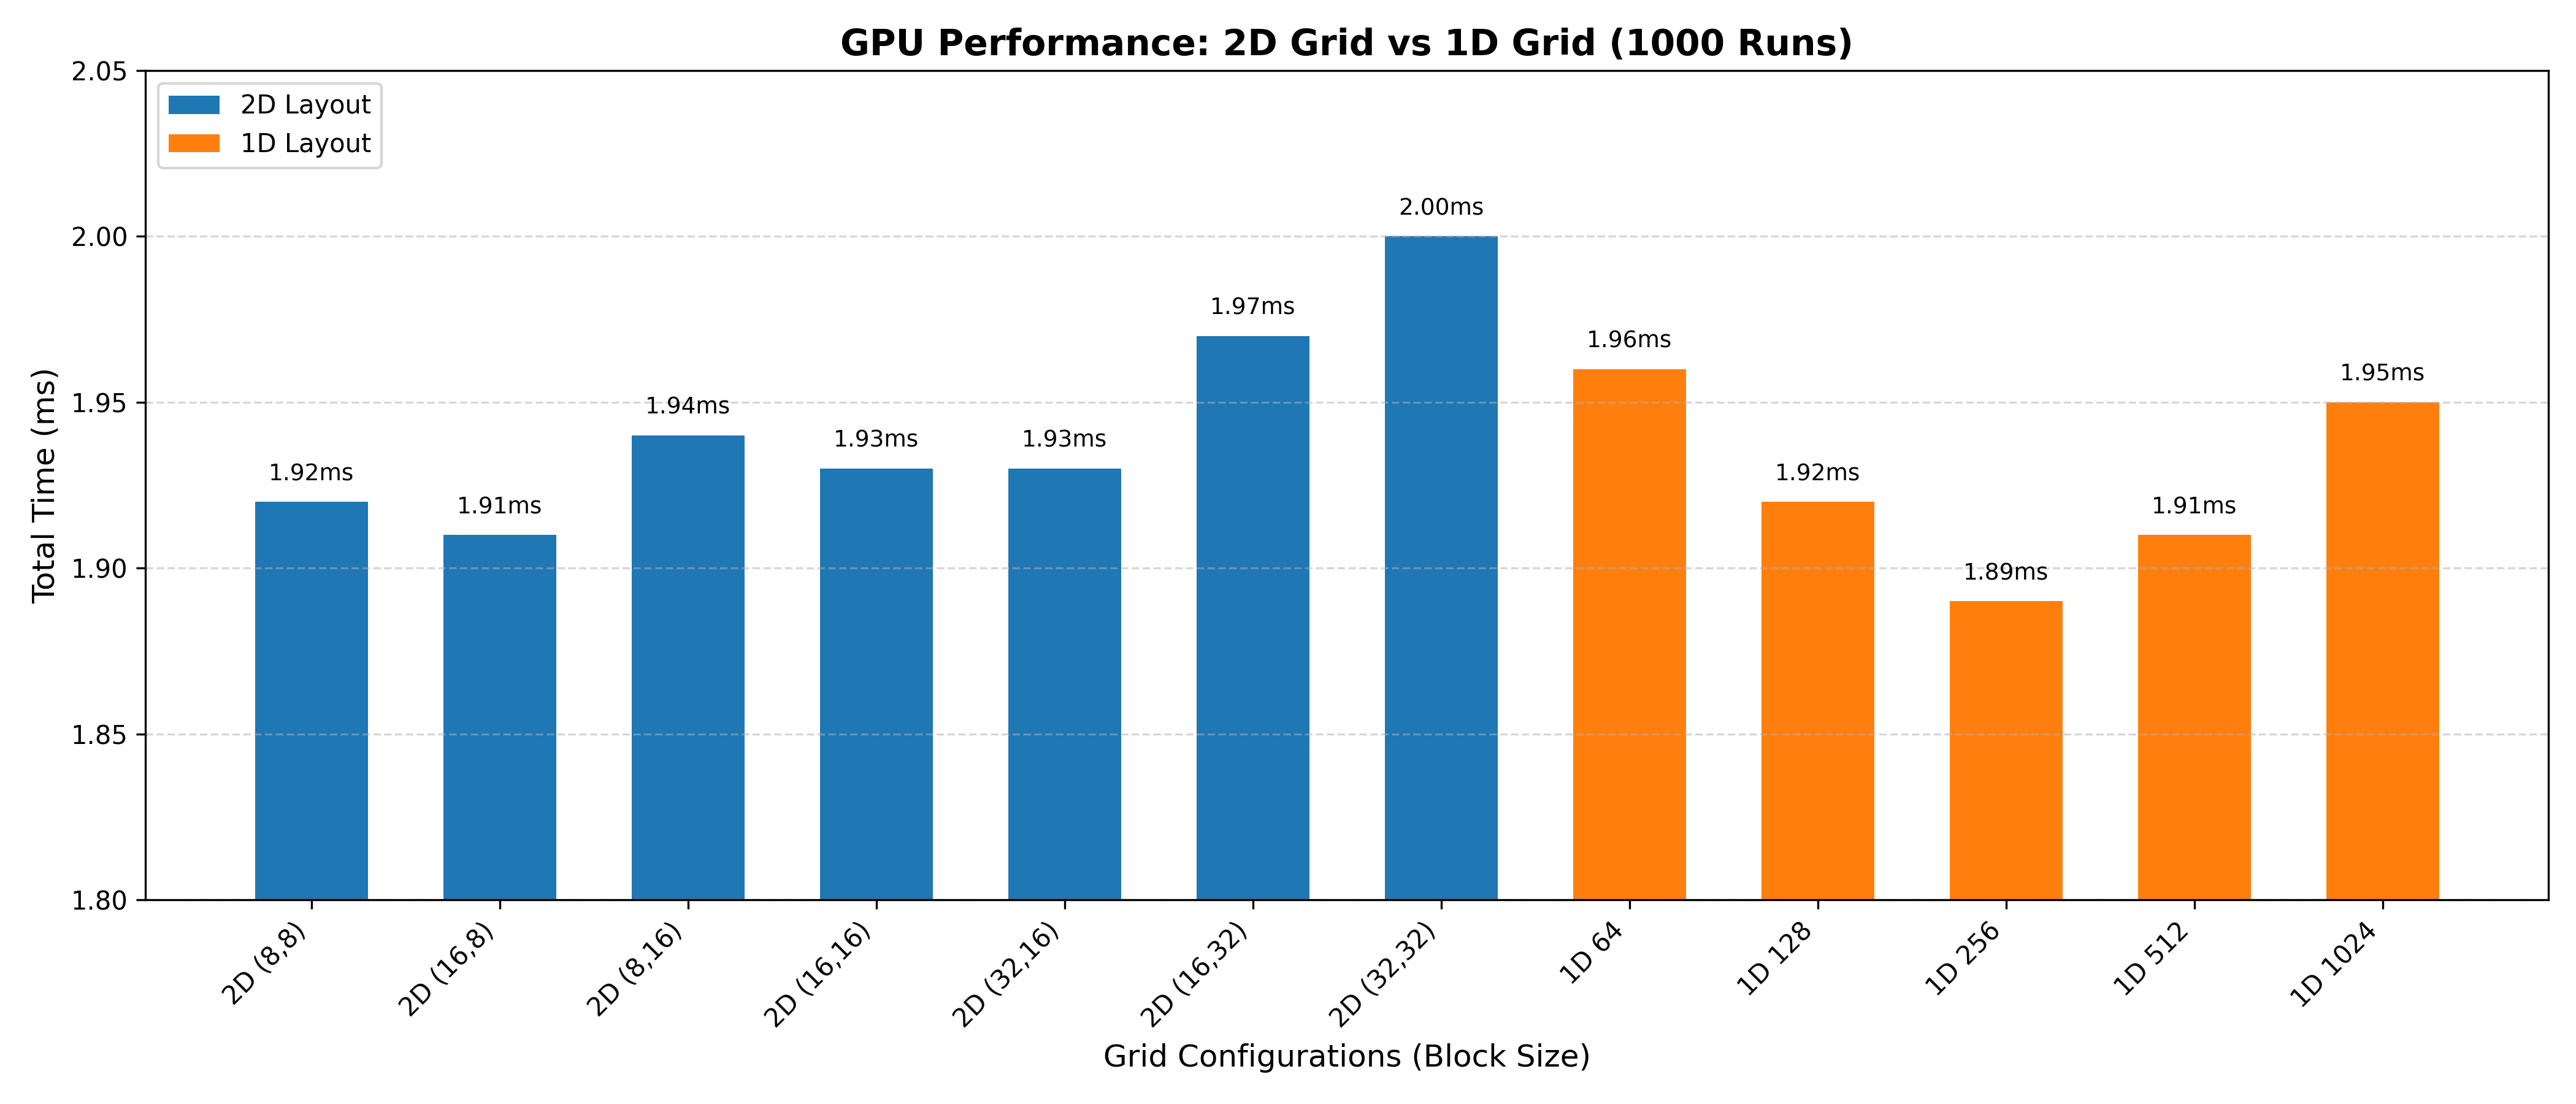
\includegraphics[width=0.75\textwidth]{grid_comparison_chart.png}
    \caption{Performance evaluation: 2D Block Layout vs. 1D Block Layout}
    \label{fig:sss}
\end{figure}

According to the benchmark data in Figure~\ref{fig:sss}, mapping the problem into a 2D layout does not yield a significant performance increase over a 1D layout. This behavior occurs because the kernel is strictly \textbf{Memory-Bound}. The arithmetic processing involved in averaging the RGB color channels is minor; consequently, the overall execution speed is bound by the hardware's global VRAM memory access and transfer bandwidth rather than the execution block topology.

\end{document}
